\documentclass[11pt,preprint, authoryear]{elsarticle}

\usepackage{lmodern}
%%%% My spacing
\usepackage{setspace}
\setstretch{1.2}
\DeclareMathSizes{12}{14}{10}{10}

% Wrap around which gives all figures included the [H] command, or places it "here". This can be tedious to code in Rmarkdown.
\usepackage{float}
\let\origfigure\figure
\let\endorigfigure\endfigure
\renewenvironment{figure}[1][2] {
    \expandafter\origfigure\expandafter[H]
} {
    \endorigfigure
}

\let\origtable\table
\let\endorigtable\endtable
\renewenvironment{table}[1][2] {
    \expandafter\origtable\expandafter[H]
} {
    \endorigtable
}


\usepackage{ifxetex,ifluatex}
\usepackage{fixltx2e} % provides \textsubscript
\ifnum 0\ifxetex 1\fi\ifluatex 1\fi=0 % if pdftex
  \usepackage[T1]{fontenc}
  \usepackage[utf8]{inputenc}
\else % if luatex or xelatex
  \ifxetex
    \usepackage{mathspec}
    \usepackage{xltxtra,xunicode}
  \else
    \usepackage{fontspec}
  \fi
  \defaultfontfeatures{Mapping=tex-text,Scale=MatchLowercase}
  \newcommand{\euro}{€}
\fi

\usepackage{amssymb, amsmath, amsthm, amsfonts}

\def\bibsection{\section*{References}} %%% Make "References" appear before bibliography


\usepackage[round]{natbib}

\usepackage{longtable}
\usepackage[margin=2.3cm,bottom=2cm,top=2.5cm, includefoot]{geometry}
\usepackage{fancyhdr}
\usepackage[bottom, hang, flushmargin]{footmisc}
\usepackage{graphicx}
\numberwithin{equation}{section}
\numberwithin{figure}{section}
\numberwithin{table}{section}
\setlength{\parindent}{0cm}
\setlength{\parskip}{1.3ex plus 0.5ex minus 0.3ex}
\usepackage{textcomp}
\renewcommand{\headrulewidth}{0.2pt}
\renewcommand{\footrulewidth}{0.3pt}

\usepackage{array}
\newcolumntype{x}[1]{>{\centering\arraybackslash\hspace{0pt}}p{#1}}

%%%%  Remove the "preprint submitted to" part. Don't worry about this either, it just looks better without it:
\makeatletter
\def\ps@pprintTitle{%
  \let\@oddhead\@empty
  \let\@evenhead\@empty
  \let\@oddfoot\@empty
  \let\@evenfoot\@oddfoot
}
\makeatother

 \def\tightlist{} % This allows for subbullets!

\usepackage{hyperref}
\hypersetup{breaklinks=true,
            bookmarks=true,
            colorlinks=true,
            citecolor=blue,
            urlcolor=blue,
            linkcolor=blue,
            pdfborder={0 0 0}}


% The following packages allow huxtable to work:
\usepackage{siunitx}
\usepackage{multirow}
\usepackage{hhline}
\usepackage{calc}
\usepackage{tabularx}
\usepackage{booktabs}
\usepackage{caption}


\newenvironment{columns}[1][]{}{}

\newenvironment{column}[1]{\begin{minipage}{#1}\ignorespaces}{%
\end{minipage}
\ifhmode\unskip\fi
\aftergroup\useignorespacesandallpars}

\def\useignorespacesandallpars#1\ignorespaces\fi{%
#1\fi\ignorespacesandallpars}

\makeatletter
\def\ignorespacesandallpars{%
  \@ifnextchar\par
    {\expandafter\ignorespacesandallpars\@gobble}%
    {}%
}
\makeatother

\newenvironment{CSLReferences}[2]{%
}

\urlstyle{same}  % don't use monospace font for urls
\setlength{\parindent}{0pt}
\setlength{\parskip}{6pt plus 2pt minus 1pt}
\setlength{\emergencystretch}{3em}  % prevent overfull lines
\setcounter{secnumdepth}{5}

%%% Use protect on footnotes to avoid problems with footnotes in titles
\let\rmarkdownfootnote\footnote%
\def\footnote{\protect\rmarkdownfootnote}
\IfFileExists{upquote.sty}{\usepackage{upquote}}{}

%%% Include extra packages specified by user
\usepackage{booktabs}
\usepackage{longtable}
\usepackage{array}
\usepackage{multirow}
\usepackage{wrapfig}
\usepackage{float}
\usepackage{colortbl}
\usepackage{pdflscape}
\usepackage{tabu}
\usepackage{threeparttable}
\usepackage{threeparttablex}
\usepackage[normalem]{ulem}
\usepackage{makecell}
\usepackage{xcolor}

%%% Hard setting column skips for reports - this ensures greater consistency and control over the length settings in the document.
%% page layout
%% paragraphs
\setlength{\baselineskip}{12pt plus 0pt minus 0pt}
\setlength{\parskip}{12pt plus 0pt minus 0pt}
\setlength{\parindent}{0pt plus 0pt minus 0pt}
%% floats
\setlength{\floatsep}{12pt plus 0 pt minus 0pt}
\setlength{\textfloatsep}{20pt plus 0pt minus 0pt}
\setlength{\intextsep}{14pt plus 0pt minus 0pt}
\setlength{\dbltextfloatsep}{20pt plus 0pt minus 0pt}
\setlength{\dblfloatsep}{14pt plus 0pt minus 0pt}
%% maths
\setlength{\abovedisplayskip}{12pt plus 0pt minus 0pt}
\setlength{\belowdisplayskip}{12pt plus 0pt minus 0pt}
%% lists
\setlength{\topsep}{10pt plus 0pt minus 0pt}
\setlength{\partopsep}{3pt plus 0pt minus 0pt}
\setlength{\itemsep}{5pt plus 0pt minus 0pt}
\setlength{\labelsep}{8mm plus 0mm minus 0mm}
\setlength{\parsep}{\the\parskip}
\setlength{\listparindent}{\the\parindent}
%% verbatim
\setlength{\fboxsep}{5pt plus 0pt minus 0pt}



\begin{document}



\begin{frontmatter}  %

\title{A Study of Covid-19}

% Set to FALSE if wanting to remove title (for submission)




\author[Add1]{Amy Visser\footnote{\textbf{Contributions:}
  \newline \emph{The data utilised in this report has been kindly
  provided by Our World in Data.}}}
\ead{}





\address[Add1]{Stellenbosch University, South Africa}


\begin{abstract}
\small{
This article aims to discuss the impact of the Covid-19 pandemic through
a variety of channels, including the experience of the pandemic on
African countries versus other regions, the impact the virus had on
specific concentrated groupings, and the effect of speed of increased
hospitalisation facilities on ICU admissions over the period.
}
\end{abstract}

\vspace{1cm}





\vspace{0.5cm}

\end{frontmatter}

\setcounter{footnote}{0}



%________________________
% Header and Footers
%%%%%%%%%%%%%%%%%%%%%%%%%%%%%%%%%
\pagestyle{fancy}
\chead{}
\rhead{}
\lfoot{}
\rfoot{\footnotesize Page \thepage}
\lhead{}
%\rfoot{\footnotesize Page \thepage } % "e.g. Page 2"
\cfoot{}

%\setlength\headheight{30pt}
%%%%%%%%%%%%%%%%%%%%%%%%%%%%%%%%%
%________________________

\headsep 35pt % So that header does not go over title




\hypertarget{introduction}{%
\section{\texorpdfstring{Introduction
\label{Introduction}}{Introduction }}\label{introduction}}

This article aims to discuss the impact of the Covid-19 pandemic through
a variety of channels, including the experience of the pandemic on
African countries versus other regions and the impact the virus had on
specific concentrated groupings.

\hypertarget{data}{%
\section{\texorpdfstring{Data \label{Findings}}{Data }}\label{data}}

\begin{figure}[H]

{\centering \includegraphics{q1_files/figure-latex/figure1-1} 

}

\caption{Covid Incidence in Africa compared to Other Regions \label{Figure1}}\label{fig:figure1}
\end{figure}

As we can see from Figure \ref{Figure1}, it appears as though Africa
experienced a relatively dampened severity of the pandemic compared to
other regions. In fact, only Oceania experienced lower case incidences
than the continent of Africa. It must be noted, however, that this may
have been due to a lack of testing facilities available on the continent
compared to other, more wealthy, continents.

\begin{table}

\caption{\label{tab:Figure2}Total Number of Cases and Deaths by Continent}
\centering
\begin{tabular}[t]{c|c|c}
\hline
continent & TotalCases & TotalDeaths\\
\hline
Africa & 11941511 & 254379\\
\hline
Asia & 154300990 & 1432514\\
\hline
Europe & 200737324 & 1847300\\
\hline
North America & 101462880 & 1448053\\
\hline
Oceania & 9332902 & 13253\\
\hline
South America & 58463479 & 1277086\\
\hline
\end{tabular}
\end{table}

While Africa's case number was high (seen in \ref{Figure2}), the deaths
are markedly lower than other continents such as Asia, Europe and North
America.

\begin{figure}[H]

{\centering 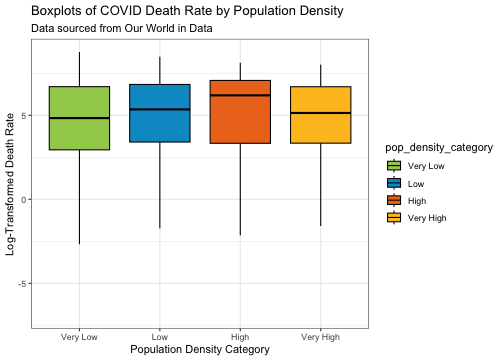
\includegraphics{q1_files/figure-latex/Figure3-1} 

}

\caption{Box Plot of Deaths by Population Density \label{Figure2}}\label{fig:Figure3}
\end{figure}

As can be seen in \ref{Figure3}, the log-transformed number of total
deaths increases as the population density increases. This, however,
appears quite marginal and even decreases for `very high'.

\begin{figure}[H]

{\centering 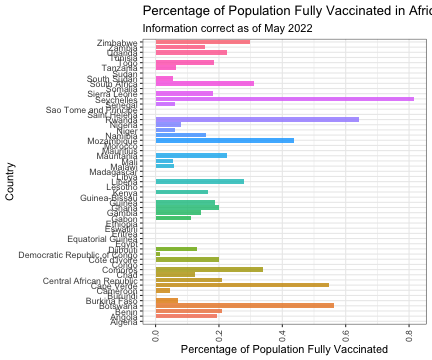
\includegraphics{q1_files/figure-latex/Figure4-1} 

}

\caption{Total Percentage of Population Vaccinated in African Countries as of May 2022\label{Figure4}}\label{fig:Figure4}
\end{figure}

Unfortunately, not all African countries posted their vaccination
statistics on a daily basis. Thus, the most recent date with the least
amount of missing data was chosen to perform an analysis on the
vaccination rate of countries within Africa. Figure 4 showcases the
percentage of the population fully vaccinated per African country,
indicating that Botswana, Rwanda and the Seychelles have the greatest
proportions of their populations vaccinated.

\begin{figure}[H]

{\centering 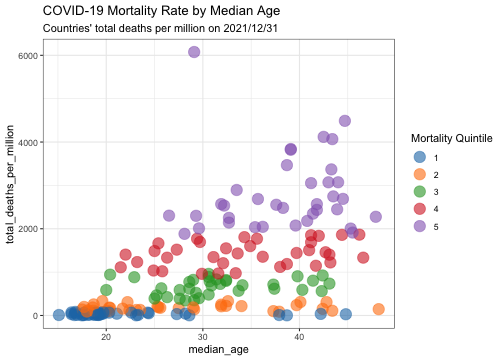
\includegraphics{q1_files/figure-latex/Figure5-1} 

}

\caption{Mortality Rate of Countries by Median Age \label{Figure5}}\label{fig:Figure5}
\end{figure}

As can be seen in \ref{Figure5}, the mortality rate spikes a lot higher
for nations with higher median ages than those with lower median ages.
This is because Covid-19 has been proven to affect the elderly at a much
higher incidence than their younger counterparts.

\hypertarget{conclusion}{%
\section{\texorpdfstring{Conclusion
\label{Conclusion}}{Conclusion }}\label{conclusion}}

This report details the effects of the Covid-19 pandemic through various
modelling techniques and decompositions. Through this, we observe that
Covid-19 disproportionately effects elderly individuals, and that Africa
was affected by the pandemic to a lesser extent than other continents.

\bibliography{Tex/ref}





\end{document}
